\chapter{Design}\label{C:des}

\section{Project Specifications and Justifications}
Given the results of the initial evaluation the project can now be constrained. It's main goals are to eliminate volume variation, control for droplet position, enable automation to reduced time between consecutive runs. It will not control, but provide data-logging for the environmental effectors; temperature, humidity, pressure. 

From this there is a number of requirements to consider:

\begin{itemize}
    \item \textbf{Mechanical Stability}:
    \item \textbf{Droplet Position Repeatability}
    \item \textbf{Consistent Volume}
    \item \textbf{Process Automation}
    \item \textbf{System Expandability}:
\end{itemize}

The project will be evaluated on its ability to control for volume and positional accuracy and repeatability as well as how it improves automation, provides environmental data and allows extension.  

\section{System Overview}

\begin{figure}[h]
    \begin{center}
        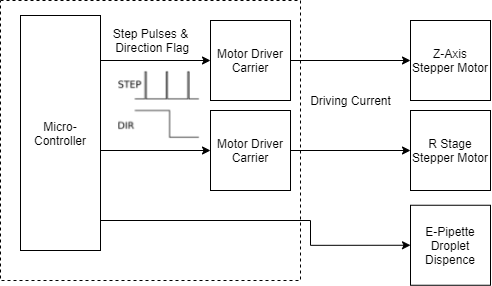
\includegraphics[width=0.5\textwidth]{img/ED_block_diag.png}
    \end{center}
\end{figure}

\section{Mechanical Design}

\begin{itemize}
    \item Discuss requirements for minimising settling time, vibrations, oscillations.overshoot of the pipette motion 
\end{itemize}

The electronic pipette formfactor is very 'organic', so the clamping mechanism to fit it to the tower plate itself was challenging to design to successfully restrict its rotation and backlash.  
The base design used to accomplish this was a 3D-printed ring clamp meant to be tightened and fit to the unique form of the pipette body. A variety of ring sizes and gap distance were printed and test fitted. From this I determined that a ring diameter of 32mm and a gap of 6mm fits and deforms to the shape of the pipette. However, there was still some rotation and slip so a notch was cut into the acrylic to slot the pipettes support rest and a second ring clamp attached lower down of the body. 


\subsection{Rotating Pipette Mount}

\begin{itemize}
    \item 3D printed pipette clamp
    \item Laser cut Tower mounted
    \item motor interface and stage fastening  
\end{itemize}

\subsection{Z micrometer Control}
\begin{itemize}
    \item Requirements: micrometer motion/extension as its turn
    \item Sliding motor shaft to knob required (2 passed)
    \item How it imposed restrictions on the system (freedom of motion)  
\end{itemize}

\begin{figure}[h]
    \centering
    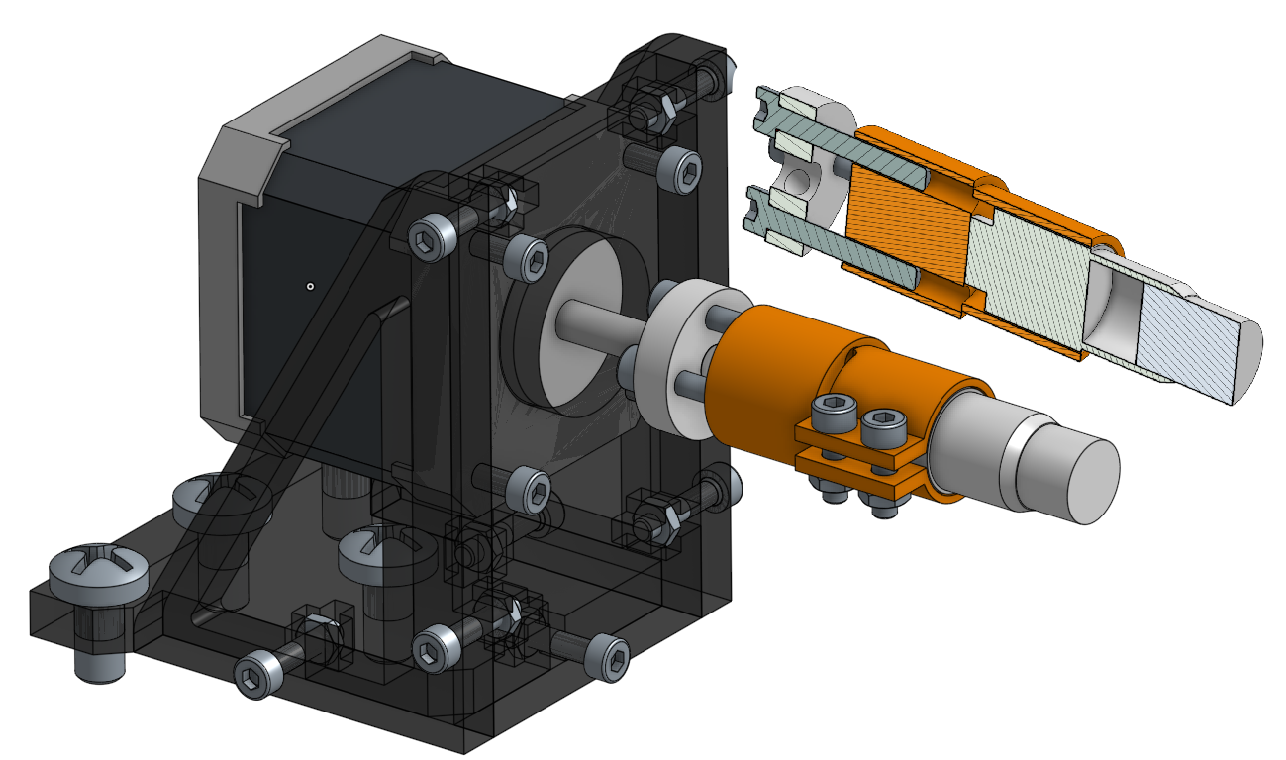
\includegraphics[width=0.4\textwidth]{img/z_control.png}
\end{figure}

\section{Electronic Design}

\subsection{Motors}
The motion required for the motors in this system is to provide rotation about the vertical axis to the mounted pipette, to swing from above the substrate to out of the camera view and over a refill reservoir, as well as continuous rotation to interface the Z axis control for droplet depositing and possible refilling.  

Stepper motors allow for both precise position control without the need for a feedback system and are capable of continuous rotation. In comparison, brushed/brushless DC motors require encoders for positional control and servos may do either but not both continuous rotation and positioning.

NEMA17 standard sized steppers were chosen to best fit the dimensions of the XYZ optical stage (60mm plate to 40mm motor frame) with room for fastening hardware. That left two choices for the top R stage motor; full size 38mm high frame or shorter pancake frame. Even through the pancake frame would reduce the overall height of the system, the shaft length available for this motor is less only 7mm and would greatly restrict the mounting options of the tower to the motor. For this reason 2 NEMA17x38mm Stepper motors were chosen. 

\subsection{Motor Driving}

\subsubsection*{The Requirements}
To drive the selected stepper motors, discrete step/direction style micro stepping drivers were chosen. This allows for the design to be flexible with its electronics placed to accommodate the experimental needs. Allows for a fairly agnostic choice for controller to supply the control signals, and standardised pinouts allow for requirement flexibility and replacements.

\begin{table}[h]
    \centering
    \begin{tabular}{|l|l|l|l|l|}
        \hline
        \textbf{}     & \textbf{A4988} & \textbf{DRV8825} & \textbf{STPIN820} & \textbf{DRV8834} \\ \hline
        Step Res      & 1/16           & 1/32             & 1/256             & 1/32             \\ \hline
        Logic Level   & 3V3/5V         & 3V3/5V           & 3V3/5V            & 3V3/5V           \\ \hline
        Current Limit & 1A             & 1.5A             & 0.9A              & 1.5A             \\ \hline
        Drive Voltage & 8-35V          & 8.2-45V          & 7-48V             & 2.5-10.8         \\ \hline
    \end{tabular}
    \caption{Comparison of considered drivers}
\end{table}

Main consideration for device choice are: micro step resolution, driving current limit (passively cooled), and configuration pinout.

\subsubsection*{The Choice}
The DRV8825 was ultimately chosen.
\begin{itemize}
    \item High microstepping resolution, lower than the STPIN820 but cheap high resolution driver are prone to step skipping \cite{step_book}
    \item Highest driving current as torque requirements are unknown for this design the headroom is nice even if it isn't use, especially as it will run cooler at lower power draw.
    \item It ranked above the DRV8834 due to it configuration pins (to set microstepping mode) as it provide all 3 pins without the requirement to leave pins floating as a setting thus allowing for full software control.
\end{itemize}

\subsection{Volume Control: ePipette}

\subsection{Environmental Monitoring}
\begin{itemize} 
    \item What will be measured?
    \item Power (battery?)
    \item Sleep the conserve
\end{itemize}
